\documentclass[11pt]{article}
\usepackage{amsmath}
\usepackage{graphicx}
\usepackage{booktabs}

\title{Figures and Tables in \LaTeX}
\author{Daily Toolkit Deep Dive --- Section 4}
\date{\today}

\begin{document}

\maketitle

\section{Inserting a figure with \texttt{graphicx}}

Figure~\ref{fig:placeholder} was generated by
\texttt{make\_placeholder\_figure.py} (a small matplotlib script) and
inserted with \texttt{\textbackslash includegraphics}. It is a
synthetic decaying curve, not a real training run --- the point of
this demo is the \LaTeX{} mechanism, not the numbers.

\begin{figure}[h]
  \centering
  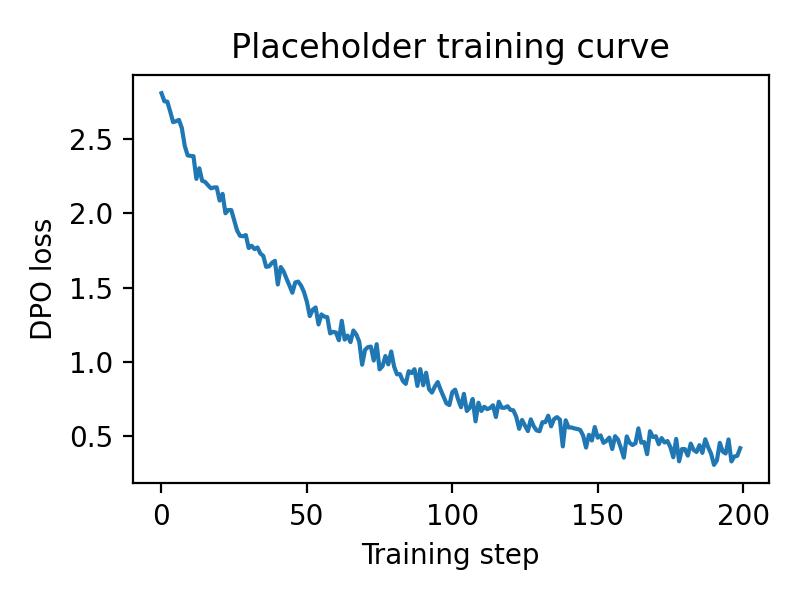
\includegraphics[width=0.6\textwidth]{placeholder-figure.png}
  \caption{A placeholder training curve generated by matplotlib and
    embedded with \texttt{graphicx}.}
  \label{fig:placeholder}
\end{figure}

\section{A three-line table with \texttt{booktabs}}

Table~\ref{tab:toy-results} uses \texttt{\textbackslash toprule},
\texttt{\textbackslash midrule}, and \texttt{\textbackslash bottomrule}
from the \texttt{booktabs} package instead of the boxed, every-cell-
has-a-border style that word processors default to. This three-line
style (three horizontal rules, no vertical rules) is the de facto
standard for tables in ML conference papers.

\begin{table}[h]
  \centering
  \caption{Toy comparison table (numbers are illustrative, not from a
    real experiment).}
  \label{tab:toy-results}
  \begin{tabular}{lcc}
    \toprule
    Method & Win rate (\%) & KL to reference \\
    \midrule
    SFT only          & 50.0 & 0.00 \\
    DPO ($\beta=0.1$) & 68.4 & 3.21 \\
    DPO ($\beta=0.5$) & 61.2 & 1.05 \\
    \bottomrule
  \end{tabular}
\end{table}

\end{document}
